\section{Pre-tokens bound merge-based extension}
\label{sec:floor}

A byte-level BPE tokenizer~\citep{sennrich-etal-2016-neural,radford2019language} first splits a string $s$ with a regex into pre-tokens $P(s)$ and then encodes each pre-token on its own by applying merges in rank order. Every pre-token yields at least one token, so $|T(s)| \ge |P(s)|$; \citet{regmi2026vowel} call this the pre-tokenization ceiling. Appending merges, whatever they are and however many, changes neither the normalizer nor the regex, so the bound holds for every tokenizer extended this way.

We turn this into a bound on the premium. For a tokenizer $T$ with pre-tokenizer $P$, the \emph{pre-token floor} is $|P(\text{ne})|/|T(\text{en})|$, the number of Nepali pre-tokens divided by the number of English tokens, summed over the 1{,}012 FLORES-200 devtest sentences. A merge-based extension that keeps $P$ and leaves English unchanged cannot bring the premium below this value, though it may stop above it. Our standard extension \RI{} leaves English unchanged: every new merge produces a token that contains a complete Devanagari code point, and since UTF-8 is self-synchronising, no new merge can fire on text without one (the same argument appears in the proof of Proposition~\ref{prop:lossless}, Appendix~\ref{app:proof}).

For today's regexes the floor is far from slack. In Llama-3 and Qwen the word branch is \texttt{[\textasciicircum\textbackslash r\textbackslash n\textbackslash p\{L\}\textbackslash p\{N\}]?\textbackslash p\{L\}+}, a run of letters optionally preceded by one other character. A Devanagari vowel sign ends the current run and becomes the leading character of the next one, so \emph{nep\=alko sark\=ar} (``government of Nepal'') becomes six pre-tokens, four of which start with a vowel sign that belongs to the previous consonant (Figure~\ref{fig:split}, Appendix~\ref{app:extras}). The floor is $2.19$ for Llama-3 and $2.17$ for Qwen3. That is above the premium of \texttt{o200k} ($1.61$), and 2.7 to 2.8 times the floor under the repaired regex of \S\ref{sec:method} ($0.79$ and $0.80$). Llama-3's premium is already $2.58$, so standard extension can lower it by at most 15\%.

\paragraph{Released extensions end at the floor.} Figure~\ref{fig:released} measures released merge-based extensions of letters-only models; Appendix~\ref{app:released} lists every number and how we found them. Ten extensions by Yamaguchi et al.\ of Llama-3, Llama-3.1, Qwen2.5 and Qwen3~\citep{yamaguchi2026lowres,yamaguchi2025elchat} cover six scripts written with combining marks. All ten end within 4\% of their floor, having closed at least 98\% of the distance from the base tokenizer.\footnote{These extensions re-order the base merges and change English token counts slightly (+6.5\% for the Llama-3 Telugu release), so for them we compare tokens with pre-tokens of the target text directly.} The 61k-token in-place expansion of LFM2 into LFM2.5~\citep{smith2026inplace} ends further from its floor ($1.07$ times it for Hindi, $1.16$ for Nepali, $1.24$ for Bengali and $1.82$ for Thai, which is written without spaces), but its floors are just as high. Under the repaired regex the same text has 2.2 to 5.9 times fewer pre-tokens, so each of these extensions stopped well short of what new vocabulary could achieve. Yamaguchi et al.'s Amharic extension, for a script without combining marks, stays at $1.57$ times its floor, and the repair does not change that floor.

\begin{figure}[t]
\centering
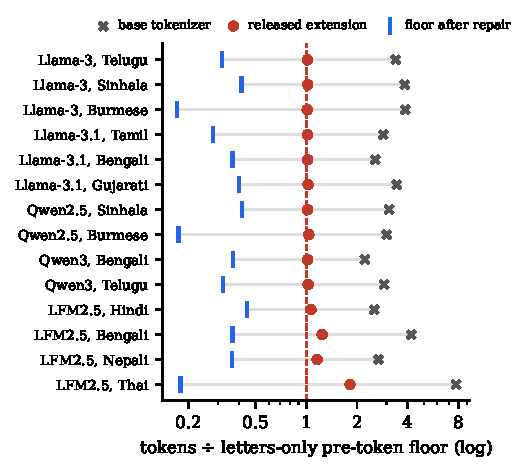
\includegraphics[width=0.95\columnwidth]{fig_released.pdf}
\caption{Released merge-based extensions of letters-only models on FLORES-200 devtest of each target language, relative to the letters-only pre-token floor. The ten extensions by Yamaguchi et al.\ (top) move from the base tokenizer ($\times$) to within 4\% of the floor (\textcolor{red}{$\bullet$}). LFM2.5 (bottom) stops further above it for Nepali, Bengali and Thai. The blue tick is the floor under the repaired regex. Full numbers, including the Amharic control, are in Table~\ref{tab:released}.}
\label{fig:released}
\end{figure}

\paragraph{Added tokens bypass the floor.} Strings registered as Hugging Face \emph{added tokens} are matched in the raw text before the regex runs, so the bound does not apply to them. SinLlama~\citep{aravinda2025sinllama} extends Llama-3 for Sinhala this way and goes below its letters-only floor. To test this route fairly, we registered as added tokens the 31{,}753 whole Devanagari strings among the 32{,}000 learned for \RII{} (\S\ref{sec:method}), on the unchanged regex. Nepali then costs $1.025$ times English on Llama-3 and $1.009$ on Qwen3, close to \RII{}'s $1.014$, and no FLORES-200 sentence without a Devanagari character changes its token ids. The floor therefore binds merge-based extension only. The price is the segmentation. Added tokens match the longest string anywhere, ignoring word boundaries, and 21\% of the matches start inside a word and 28\% end inside one. Allowing only whole-word matches (\texttt{single\_word=True}) removes those splits and also the gain: the premium returns to $2.49$ on Llama-3 and $4.22$ on Qwen3 (Appendix~\ref{app:extras}). We did not train models with added tokens.
